\section{Описание практической части}
\label{sec:Section4} \index{Section4}

\subsection{Драйверы Linux для управления тактовой частотой ядра процессора Gem5}

    Для построения модели производительности и реализации политики регулирования частот центрального процессора
    необходимо реализовать драйвер управления тактовыми частотами в ядре Linux. Интерфейсы, позволяющие регулировать
    тактовые частоты как в пространстве пользователя, так и пространстве ядра в Linux версии 6.1 уже
    реализованы в драйвере $cpufreq$, остаётся реализовать низкоуровневую часть, связанную непосредственно
    с устройством взаимодействия Linux и Gem5.

    В Gem5 уже присутствуют механизмы, позволяющие изменять тактовые частоты многих устройств. Любой
    класс, являющийся наследником класса $ClockedObject$, способен регулировать тактовые частоты своих
    объектов, если их реализация зависит от этих частот. Например, класс $BaseCPU$, описывающий
    абстрактное ядро процессора, является наследником $ClockedObject$ использует параметры
    тактовой частоты для управления производительностей работы конвейера и внутренних вычислительных блоков.

    В Gem5 существует контроллер, регулирующий тактовые частоты всех устройств во время симуляции --
    $EnergyController$. Несмотря на то, что, как правило, параметры внутреннего устройства компьютерной
    системы, на которой запускается ядро Linux, передаются в ядро через $device \; tree$ файлы (\cite{KernelDocsDTS}),
    в Gem5 реализованы интерфейсы в виде дополнительных регистров, значения в которых изменяются
    в зависимости от способов обращения к ним: даже при чтении регистра его состояние может измениться.
    $EnergyController$ осуществляет контроль доступа к таким регистрам, посылая уведомление о
    необходимости изменения тактовой частоты нужному устройству (или его контроллеру) в системе
    в зависимости от команд и регистров, к которым произошло обращение.

    \begin{figure}[!h]
        \caption{Схема взаимодействия Gem5 и драйверов Linux}
        \centering
        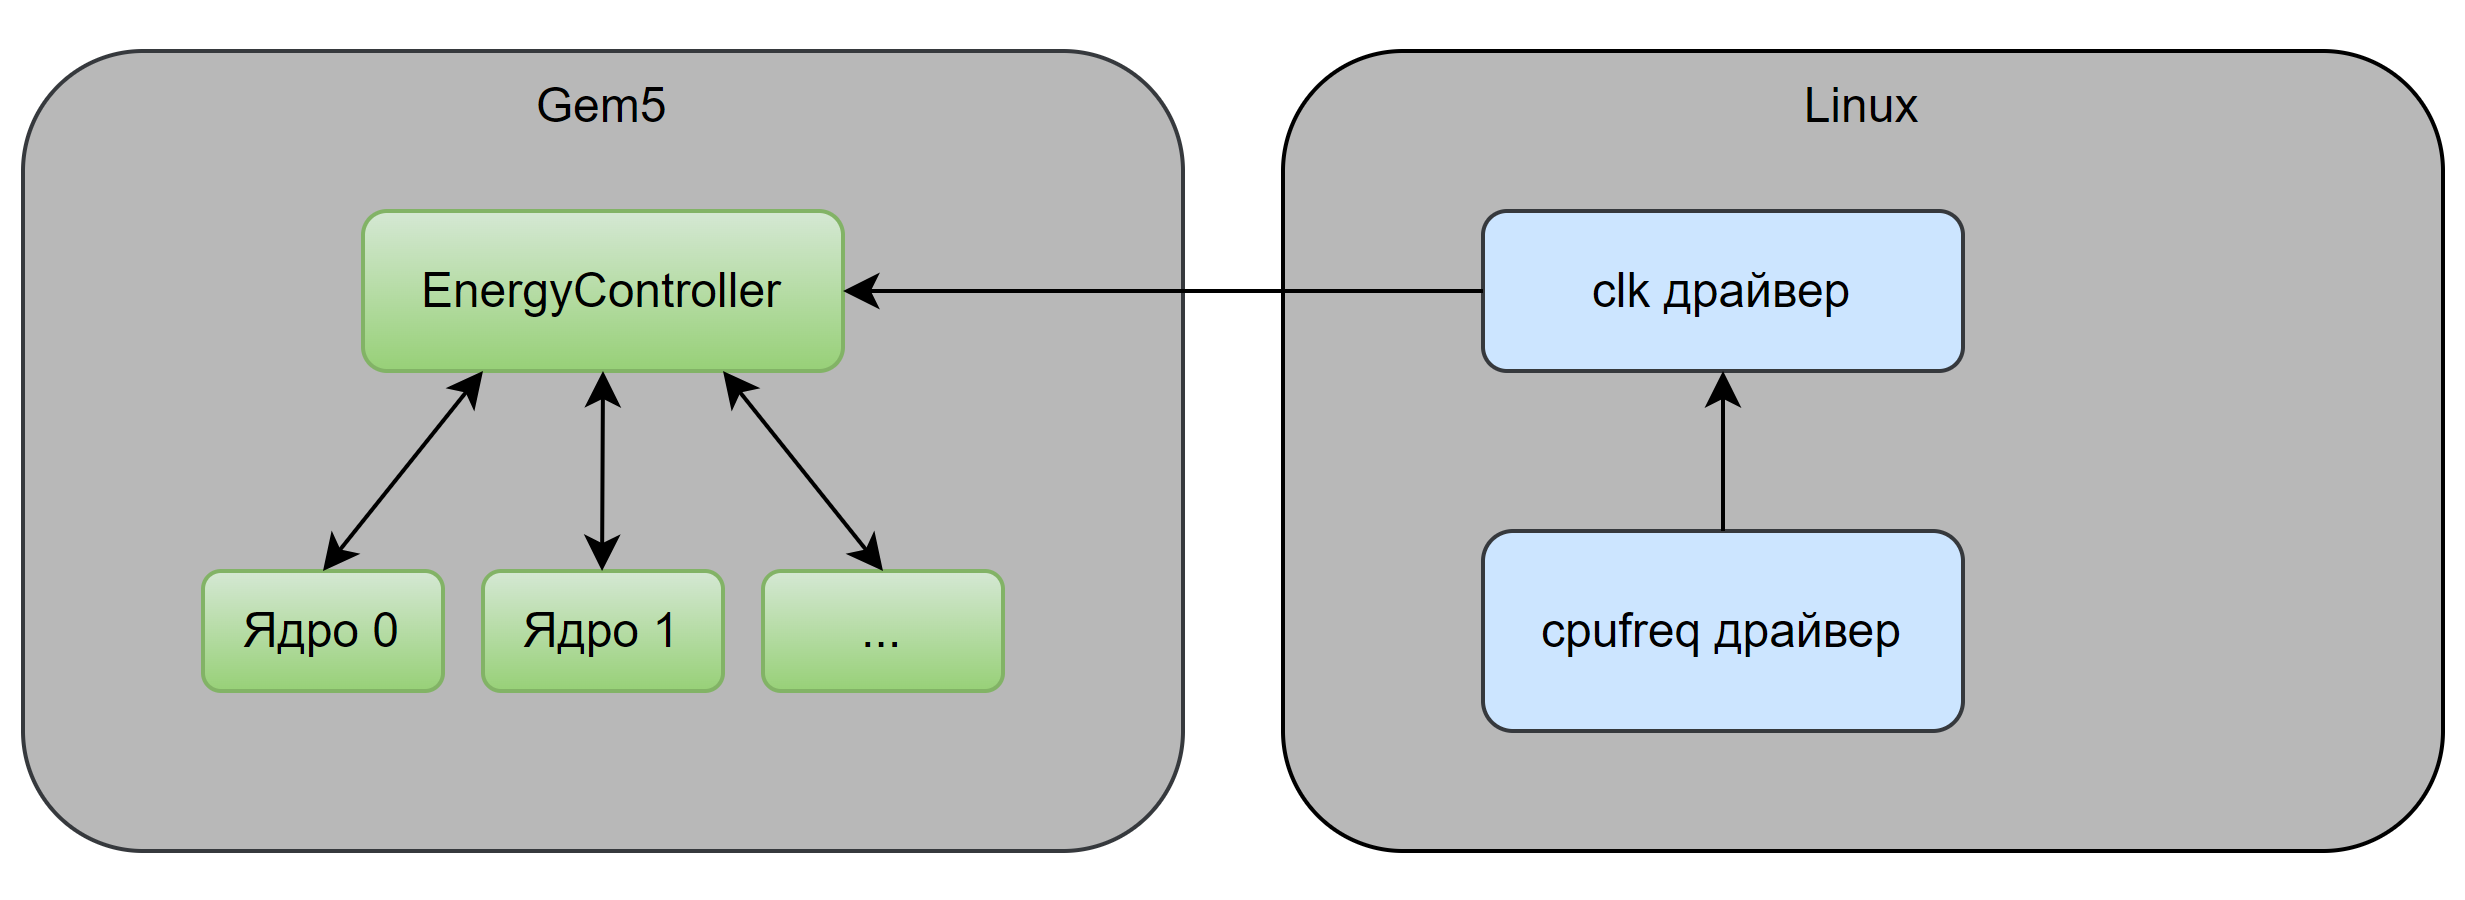
\includegraphics[width=145mm]{gem5_cpufreq}
        \label{gem5_cpufreq}
    \end{figure}

    Дополнительные регистры для внешнего взаимодействия с $EnergyController$ из ядра Linux с помощью
    $device \; tree$ переведены с соответствующий диапазон физических адресов, которым во время запуска ядра
    Linux ставятся в соответствие виртуальные адреса через таблицу виртуальных страниц.

    В ядре Linux существует дополнительный интерфейс-драйвер $clk$ для описания устройств (как
    настоящих, так и виртуальных), в котором необходимо реализовать низкоуровневое
    взаимодействие с регистрами, контролирующими тактовые частоты, по физическим адресам.
    Чтобы $cpufreq$ мог контролировать тактовые частоты своими интерфейсами, необходимо написать собственную
    реализацию ряда функций, которые будут использовать реализацию $clk$ драйвера для управления
    тактовыми частоты.

    Таким образом, был реализован интерфейс драйвера $clk$ для взаимодействия с $EnergyController$
    в симуляторе Gem5 и интерфейс драйвера $cpufreq$, использующий реализацию $clk$ для возможности
    регулировать тактовые частоты. Схема взаимодействия компонент представлена на рис. \ref{gem5_cpufreq}.

\subsection{Реализация счётчиков микроархитектурных событий, связанных с кешами} \label{counters_impl}

    Из главы \ref{model_counters} следует, что необходимо использовать счётчики микроархитектурных
    событий $CPU\_CYCLES$, $INST\_RETIRED$ и события, связанные с кешами $L1I\_CACHE\_REFILL$,
    $L1D\_CACHE\_REFILL$ и $L2D\_CACHE\_REFILL$, которые не реализованы в Gem5, как и все остальные счётчики,
    связанные с кешами.

    Так как кеши в Gem5 реализованы как абстрактные устройства посредством классов в С++, кеши,
    разделяемые между несколькими ядрами, должны уметь распознавать источник возникновения транзакции,
    проводимой с кешом. Например, в процессоре с 2-мя уровнями кешей при перезаполнении кеш-линии со
    стороны ОЗУ из-за промаха в кеш счётчик микроархитектурных событий $L2D\_CACHE\_REFILL$
    необходимо увеличить именно для того ядра, от которого изначально произошёл промах в кеш.

    Политика регулирования тактовых частот в Linux будет реализована для процессора с 3-мя,
    а не 2-мя уровнями кешей (2 уровня были рассмотрены лишь для примера), поэтому вместо счётчиков
    $L1I\_CACHE\_REFILL$ и $L1D\_CACHE\_REFILL$ необходимо брать в рассмотрение $L3D\_CACHE\_REFILL$,
    т.к. 2-ой уровень кеша оперирует с тактовой частотой процессора, поэтому его можно не рассматривать
    (аналогично тому, как были убраны из рассмотрения кеши 1-ого уровня в главе \ref{model_chapter}).

    В Gem5 транзакции с устройствами и шинами, их соединяющими, происходят с помощью пакетов,
    внутри которых содержится информация об исходном отправителе на протяжении всего пути
    пакета. Таким образом, требуется перехватить пакет в месте, где происходит само микроархитектурное
    событие, и, если инициатором транзакции (отправитель пакета) является ядро процессора,
    увеличить счётчик для этого ядра в соответствии с типом пакета (дял некоторых типов пакета и вовсе
    ничего не требуется увеличивать).

    В Gem5 для архитектуре ARM64 уже реализованы все архитектурные регистры (счётчики), предназначенные
    для работы с микроархитектурными событиями, а в Linux драйвер $perf$ уже реализует функционал,
    позволяющий использовать такие счётчики как из пространства ядра, так и из пространства пользователя.

    Таким образом, были реализованы механизм распознавания инициатора транзакции, проводимой
    с кешем, и увеличения счётчиков микроархитектурных событий в зависимости от типа транзакции
    для ядра-инициатора.

\subsection{Вычисление коэффициентов для модели производительности ядра процессора} \label{model_coeffs}

    Чтобы найти численные значения $C_{L_2}$ и $C_{ram}$ (см. главу \ref{model_chapter}) в формуле

    \begin{equation*}
        cpi = cpi_{cpu}^{L_1} + \alpha^{par} \cdot
        \left( C_{L_2} \cdot npi_{L_2} + C_{ram} \cdot npi_{ram} \right) \cdot freq_{cpu},
    \end{equation*}
    необходимо измерить значения $cpi$, $npi_{L_2}$, $npi_{ram}$ для различных тактовых частот
    $freq_{cpu}$ для определённого набора рабочих нагрузок (приложений). Так как значение $cpi_{cpu}^{L_1}$
    находится динамически по формуле \eqref{cpi_l1_sum}, то его мы будем игнорировать. Так как
    по-умолчанию $\alpha^{par} = 1$, это же значение будет взято для вычисления остальных коэффициентов.

    Как уже было упомянуто в главе \ref{counters_impl}, в финальной реализации политики регулирования тактовых
    частот будет система 3-мя уровнями кешей и следующей формулой:
    \begin{equation} \label{cpi_formula_3lvl}
        cpi = cpi_{cpu}^{L_2} + \alpha^{par} \cdot
        \left( C_{L_3} \cdot npi_{L_3} + C_{ram} \cdot npi_{ram} \right) \cdot freq_{cpu},
    \end{equation}
    поэтому находится будут коэффициенты $C_{L_3}$ и $C_{ram}$. Все формулы, расммотренные в предыдущих
    главах, остаются применимы, за исключением замены $cpi_{cpu}^{L_1}$ на $cpi_{cpu}^{L_2}$,
    $C_{L_2}$ на $C_{L_3}$ и $npi_{L_2}$ на $npi_{L_3}$.

    В качестве ядра процессора будет использоваться ядро HPI (High Performance In-order)
    \cite{gem52017HPI} без спекулятивного выполнения инструкций. Размеры кешей инструкций и данных
    1-ого уровня -- 32 Кб, 2-ого уровня -- 512 Кб, 3-его уровня -- 4 Мб.

    Величины $npi_{L_3}$ и $npi_{ram}$ являются инвариантами для рассматриваемых бенчмарков, т.е.
    график зависимости $cpi(freq_{cpu})$ является графиком полинома 1-ой степени ($npi_{L_3}$ и
    $npi_{ram}$ не зависят от тактовой частоты), поэтому значения
    $C_{L_3}$ и $C_{ram}$ могут быть найдены
    применением линейной регресcии к формуле \eqref{cpi_formula_3lvl} для каждого бенчмарка.
    График зависимости приведён на рис. \ref{pic:cpi_model}.

    Набор приложений должен быть таким, чтобы часть приложений полностью попадало в кеши 1-ого и 2-ого уровней,
    часть совершало промах во 2-ой уровень, но попадание в 3-ий, и остальная часть совершала промах в 3-ий уровень
    кеша, из-за чего происходит обращения в DDR (ОЗУ). Для таких целей возможно использование параметризованного
    бенчмарка, который рандомизированно обращается в диапазон некоторого массива, а диапазон итеративно меняется так,
    чтобы через какое-то количество итераций все диапазоны были пройдены.

    Предлагается ко вниманию следующий параметризованный бенчмарк, генерирующий набор бенчмарков

    \begin{lstlisting}
        unsigned long seed = 123456789;
        unsigned long a = 6364136223846793005;
        unsigned long c = 1442695040888963407;

        static int ARRAY[ARRAY_SIZE];

        unsigned long rand_number()
        {
            seed = a * seed + c;
            return seed;
        }

        int main()
        {
            for (unsigned long iter = 0; iter < N_ITERS; ++iter) {
                unsigned long idx = SHIFT * iter + (rand_number() % SHIFT);
                ARRAY[idx % ARRAY_SIZE] = ARRAY[(ARRAY_SIZE - idx) % ARRAY_SIZE];
            }

            return 0;
        }
    \end{lstlisting}

    В качестве функции генерации случайных чисел был использован линейный конгруэнтный генератор,
    предложенным Дональдом Кнутом \cite{knuth1973art}, параметры $ARRAY\_SIZE$ и $SHIFT$ определяют
    поведение бенчмарка, параметр $N\_ITERS$ никакого значения не играет и может быть выбран любым
    (но достаточно большим).

    \begin{figure}[!h]
        \caption{График зависимости $cpi(freq_{cpu})$ для набора бенчмарков}
        \centering
        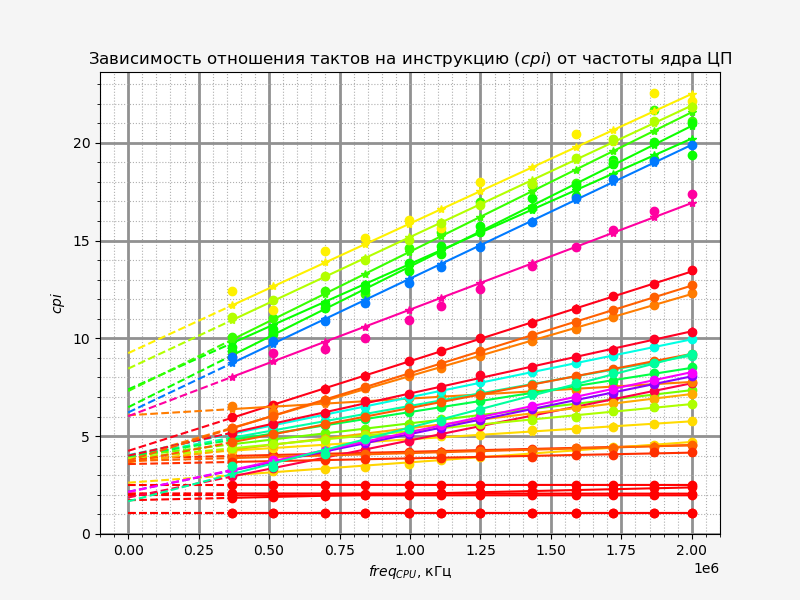
\includegraphics[width=139mm]{CPI_model}
        \label{pic:cpi_model}
    \end{figure}

    \begin{figure}[!h]
        \caption{График 3D зависимости $lat_{gen}(npi_{L_3}, npi_{ram})$}
        \centering
        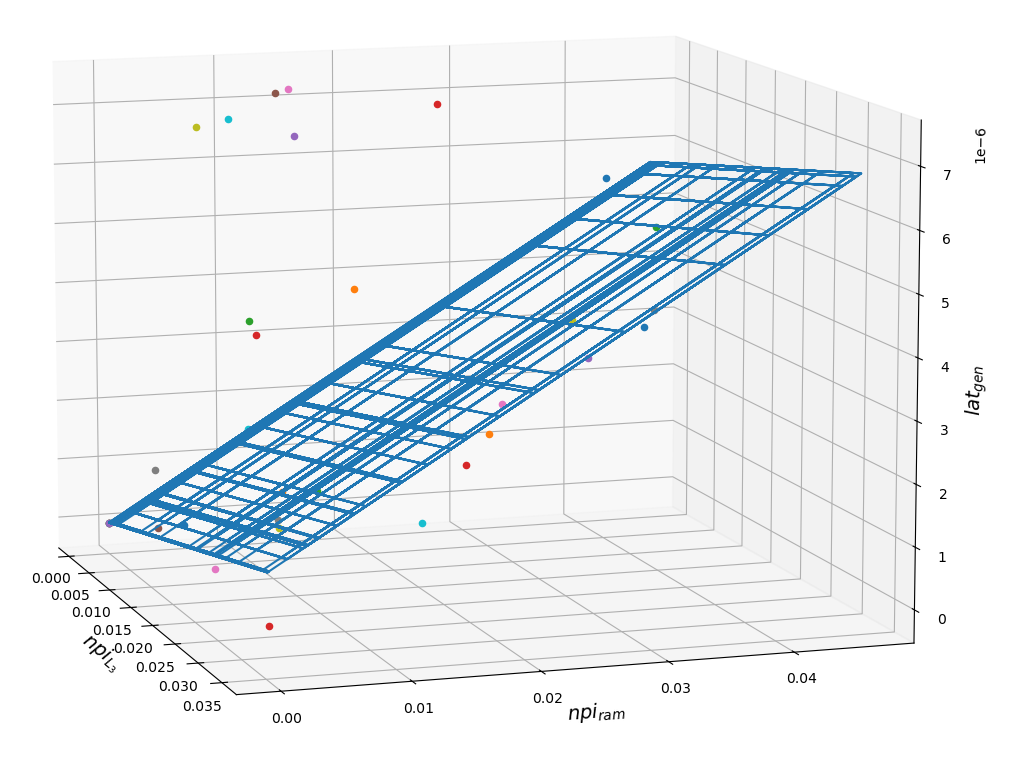
\includegraphics[width=139mm]{CPI_model_2}
        \label{pic:cpi_model_2}
    \end{figure}

    Из зависимости $lat_{gen}(npi_{L_3}, npi_{ram})$ можно извлечь значения $C_{L_3}$ и $C_{ram}$ --
    график приведён на рис. \ref{pic:cpi_model_2} (плоскость соответствует линейной
    зависимости). Из графика можно наблюдать, что не существует явного вида зависимости
    $lat_{gen}(npi_{L_3}, npi_{ram})$, так как существуют дополнительные факторы, такие коэффициент
    параллелизма в память, который индивидуален для каждого приложения. Принимая $\alpha^{par} = 1$,
    найдём усреднённые значения $C_{L_3}$ и $C_{ram}$ из линейной регрессии:

    \begin{equation}
        C_{L_3} = 3.26727 \cdot 10^{-5} \; \text{кГц}^{-1}, \; C_{ram} = 1.22416 \cdot 10^{-4} \; \text{кГц}^{-1}.
    \end{equation}

\subsection{Реализация политики регулирования тактовых частот в ядре Linux}

    Реализация политики регулирования тактовых частот подразумевает реализацию следующих компонент:
    \begin{enumerate}
        \item Модуль, собирающий статистику микроархитектурных событий для каждого потока исполнения
        и ядра процессора (событий, описанных в главе \ref{model_coeffs}).
        \item Модуль, вычисляющий утилизацию для каждого потока исполнения и ядра процессора по формуле
        \eqref{util_sum_final}, регулирующий параметр $\alpha^{par}$ по формулам \eqref{alpha_regul_formula}
        и \eqref{alpha_res_formula}, а также выбирающий тактовую частоту ядра по формуле
        \eqref{optimal_cpufreq}.
        \item Модуль, выставляющий максимальную тактовую частоту среди выбранных с помощью модели
        для каждого ядра в ядерном кластере (т.к. тактовые частоты могут выставляться только целиком
        для всего кластера).
    \end{enumerate}

    В качестве промежутка времени $\tau$, использованном во всей работе, выбран квант времени планировщика,
    равный $CONFIG\_HZ$, настраиваемый в конфигурации ядра Linux. В конфигурации выставлено значение
    $CONFIG\_HZ = 100$, что означает частоту $100$ Гц, то есть квант времени $\tau = 10$ мс.

    Обновление статистики микроархитектурных событий необходимо фиксировать при следующих событиях:
    \begin{enumerate}
        \item По таймеру каждые $\tau$ мс в функции \lstinline{scheduler_tick(void)}.
        \item В функции \lstinline{perf_rotate_context(struct perf_cpu_context *cpuctx)} при ротации
        закреплённых микроархитектурных событий (если количество измеряемых событий
        превышает количество физически доступных счётчиков, часть событий можно открепить, чтобы измерения по ним
        чередовались на одном счётчике и собирали менее точную усреднённую статистику).
        \item В функции \lstinline{context_switch(struct rq *rq, ...)} при смене контекста исполнения на
        ядре процессора.
    \end{enumerate}

    Выставление тактовой частоты ядер необходимо совершать при следующий событиях:
    \begin{enumerate}
        \item По таймеру каждые $\tau$ мс в функции \lstinline{scheduler_tick(void)} (после обновления статистики
        счётчиков микроархитектурных событий).
        \item В функции \lstinline{finish_task_switch(struct task_struct *prev)} при пробуждении ядра
        (перехода из состояния сна в активное) и назначении потока исполнения.
        \item В функции \lstinline{set_task_cpu(struct task_struct *p, unsigned int new_cpu)} в случае миграции
        потока исполнения на новое ядро процессора.
    \end{enumerate}

    С коэффициентами $\gamma = 0.8$ в формуле \eqref{optimal_cpufreq} и $\beta = 0.8$ \eqref{alpha_res_formula}
    тестирование на искусственном бенчмарке, основу которого составляет комбинация бенчмарков, приведённых в
    главе \ref{model_coeffs}, приводит к результатам в виде уменьшения энергопотребления на $6.4\%$. Измерение
    энергопотребление было внедрено в Gem5 в виде формулы для мощности энергопотребления $P = C \cdot V^2 \cdot freq_{cpu}$,
    где ёмкость $C$ считалась равной константой, а напряжение смоделировано формулой
    $V = V_0 \sqrt{\frac{freq_{cpu}}{freq_{cpu}^{min}}}$.

    Анализ оптимизации производительности требует отдельного исследования, т.к. его нужно проводить для значительно
    большего количества бенчмарков с различными спецификами исполнения. В среднем на $1$ секунду симуляции приходится
    порядка $2000-4000$ секунд, это означает, что для тестирования $10$ бенчмарков, каждый из которых длиться
    по $100$ секунд в симуляции, необходимо 41 сутки только для измерения данных, что затруднительно выполнить
    в данной работе.

\newpage
